\chapter{Linies de transmissió}

\section{Teoria de paràmetres distribuïts}

Les línies de transmissió són un tipus de guia d' ones que transporta quasi exclusivament el mode TEM. Aquest mode necessita dos conductors diferentment carregats per a propagar-se: en cas contrari el potencial és nul en l' interior i $\vec E$ és constant; com que a les parets $\vec E = 0$ el camp seria nul en tota la guia. Les LT estaran sempre formades per dos conductors. Un bon exemple és la línia coaxial, que són dos conductors de secció circular concèntrics i separats per un dielèctric.

 Com que $\del _t \vec e_t = \del _t \vec h_t = 0 $, podem utilitzar mètodes d' estàtica (mètode de les imatges, teorema d' Ampère...). Per a utilitzar teoria del potencial cal que definim dos punts, un amb $Q^+$ i un amb $Q^-$, que seran els dos conductors. Recordem que al TEM tenim una freqüència espacial proporcional a la freqüència $\beta = \omega \sqrt{\mu \epsilon } $, el que significa que no hi ha freqüència de tall i que $v_f = \frac{\omega}{\beta} = \frac{1}{\sqrt{\omega\epsilon}} = \frac{c}{\sqrt{\epsilon _ r \omega _r}}$, $v_g = v_f$ (si $\epsilon \neq f(\omega)$) i que $\vec e_ \sigma = -Z \sub{TEM} \uz \times \vec h _ \sigma$.

Per a facilitar l' estudi de les LT anem a passar de 4 quantitats (els quatre camps restants) a dos:  $V(z)$ i $I(z)$. Si $ \vec h$ i $\vec e$ són $\sim e ^{jwt}$ aleshores $I$ i $V$ també ho seran, i les quantitats a l' eixida seran una modificació  de les de l' entrada. Com que els elements dels circuits elèctrics (condensadors, bobines, resistències i conductàncies) tenen aquest mateix efecte tractarem cada secció $\Delta z$ de la guia com un circuit (\cref{fig:circuit}).

\begin{figure}[h]
  \centering
  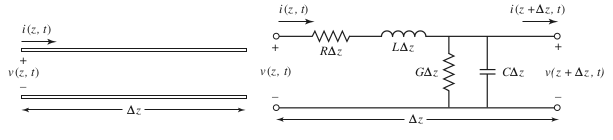
\includegraphics[scale=0.6]{circuitequivalent}
  \caption{Circuit equivalent d' una línia de transmissió}
  \label{fig:circuit}
  \vspace{-1 em}
\end{figure}

\subsection{Capacitat}

Els dos conductors de la línia formen un condensador amb càrrega $Q$ i tensió $V$, amb capacitància total $\mathcal C = \frac{Q}{V}$. Com que la cárrega és proporcional a la longitud de la guia $l$ podem definir la capacitat per unitat de longitud $C = \frac{\mathcal C}{l} = \frac{Q}{l V}$.

\subsection{Inductància}

Considerem el circuit rectangular format per dos línies al llarg dels conductors i dos linies entre els conductors a l' entrada i a l' eixida (vore figura). El flux a través d' aquesta secció del camp magnètic creat pels corrents als conductors forma una autoinductància $\mathcal L = \frac{\phi}{I}$, que al igual que la capacitància és proporcional a la longitud de la línia i dona lloc a una autoinductància distribuïda $L = \frac{\mathcal L}{l} = \frac{\phi{}}{l I}$

\subsection{Conductància}

Si el dielèctric té pèrdues, caracteritzades per $\epsilon _r $, $\sigma \sub D\neq \infty$, existirà una corrent de pèrdues en la direcció radial $\vec J = \sigma \sub D\vec E$. La conductància d' aquesta corrent és $\mathcal G = \frac{1}{R} = \frac{I \sub {pèrdues}}{V} = \frac{\int \vec J \sub{pèrdues} d \vec S}{V} = \frac{\int \sigma \sub D\vec E d \vec S}{V} = \frac{\sigma _D}{V} \int \vec E d \vec S$. Com que la integral és calcula sobre un cilindre concèntric als conductors tindrem $\mathcal G \propto l$, i definim $G = \frac{\mathcal G}{l}$

\subsection{Resistència}

Com que la conductància dels conductors és alta però no infinita tindrem pèrdues en aquests, determinades per la seua resistència superficial $R_s$. Sabem del tema anterior que les pèrdues han de ser $P_p = \frac{1}{2} R_s \int \vert \vec H \sub{sup} \vert dS$. Com que en teoria de circuits la potència dissipada per una resistència és $\frac{1}{2} \vert I \vert ^2 \mathcal R$, la resistència equivalent de la línia és $\mathcal R = \frac{R_s}{\vert I \vert ^2} \int \sub {cond} \vert \vec H  \vert dS$, i al ser la integral sobre els conductors proporcional a $l$ definim $R = \frac{\mathcal R}{l}$.

\section{Ones de tensió i corrent}

Cada element $\Delta z$ de la línia, per tant, pot ser tractat com un circuit amb dos fils (un per cada conductor) i el elements circuitals apropiats, com es mostra a la figura. L' ordre dels elements és irrellevant.

Ara podem utilitzar teoria de circuits per a estudiar el comportament de la diferència de potencial entre els dos conductors/fils $V(z, t)$ i la corrent que circula per aquests $I(z, t)$. Al llarg de $\Delta z$ els elements del circuit modificaran aquestes quantitats:
\begin{subequations}
  \begin{align}
    V(z) - V(z + \Delta z) &= I(z) (j L \omega \Delta z + R \Delta z) \\
    I(z) - I(z + \Delta z) &= V(z + \Delta z) (j \omega C \Delta z t + G \Delta z)
  \end{align}
\end{subequations}

Si dividim entre $\Delta z$ i fem el limit $\Delta z \to 0$ obtenim dues equacions diferencials acoblades, anomenades equacions del telègraf:
\begin{subequations}
  \begin{align}
    - \frac{dV}{dz} &= I(z)(j\omega L + R ) \label{diffV} \\
    - \frac{dI}{dz} &= V(z)(j\omega C + G )
  \end{align}
\end{subequations}

Definint $Z = R + j \omega L $ i $ Y = G + j \omega C$ i derivant ambdues entre $z$ les desacoblem i obtenim les solucions, que resulten ser dues ones.
\begin{subequations}
  \begin{align}
    V = V _0 e^{j \omega t}e^{\pm \sqrt{ZY} z} \label{solV}\\
    I = I _0 e^{j \omega t}e^{\pm \sqrt{ZY} z} \label{solI}
  \end{align}
\end{subequations}


\section{Relació entre tensió i corrent}

Si $V$ està relacionada amb $H$, $I$ està relacionada amb $\vec E$, i $\vec E$ amb $\vec H$, ha d' existir una relació entre $V$ i $I$. Substituint \cref{solV,solI} en \cref{diffV} obtenim
\begin{equation}
  \frac{V}{I} = \pm\sqrt{\frac{Z}{Y}} = \pm\sqrt{\frac{R+j\omega L}{G + j\omega C}} = \pm Z_c
\end{equation}
On $Z_c$ és una quantitat complexa amb dimensions de resistència, que s' anomena impedància característica de la línia, ja que sols depén de les propietats físiques d' aquesta. El signe positiu correspon a la $Z_c$ que afecta a la ona que viatja en el sentit $+z$, i el negatiu a la que va cap a $-z$. Si connectem dues línies la diferència entre les $Z_c$ pot provocar reflexions no desitjades, pel que totes les linies de transmissió operen a 50 $\Omega $.

\section{Factor de propagació}

El factor de propagació de les ones de tensió i corrent, $\gamma = \sqrt{ZY}$, és un número complex, les parts real i imaginària del qual estan relacionades amb l' atenuació exponencial i la ondulació, respectivament.
\begin{equation}
  \sqrt{ ZY }= \sqrt{(R + j \omega L)(G + j\omega C)} = \frac{\alpha}{2} + j \beta
\end{equation}

Estudiem aquests dos termes en casos importants.

\subsection{Línia sense pèrdues}

En una línia sense pèrdues $R = G = 0$, pel que $\gamma = \sqrt{j\omega Lj\omega C} = j\omega \sqrt{LC}$, i les ones tindran freqüència $\beta = \omega \sqrt{LC}$, i $v_f = v_g = \frac{1}{\sqrt{LC}}$. Aquestes línies tenen $Z_c = \sqrt{\frac{L}{C}}$.

\subsection{Línia amb poques pèrdues}

Si $R << \omega L$ i $G << \omega C $ podem obtindre una expressió aproximada per a les parts reals i imaginària de $\gamma$ expandint fins a segon ordre (si sols utilitzem primer ordre els resultats són els mateixos que en el cas anterior):
\begin{subequations}
  \begin{align}
   \gamma &= \sqrt{(R + j\omega L)(C + j\omega C)} = \sqrt{\frac{j\omega L }{j\omega C}}  \sqrt{\left ( 1 +  \frac{R}{j\omega L} \right) \left ( 1 + \frac{G}{j\omega C } \right )}  \\
   &\approx \frac{\sqrt{LC}}{2} \left ( \frac{R}{L} + \frac{G}{C} \right ) \left [ 1 - \frac{1}{8 \omega ^2} \left ( \frac{R}{L} - \frac{G}{C} \right ) ^2 \right ] + j \omega \sqrt{LC} \left [ 1 +  \frac{1}{8 \omega^2} \left ( \frac{R}{L} - \frac{G}{C} \right) ^2 \right ] \nonumber
  \end{align}
 
\end{subequations}

Com que la freqüència de la ona $\omega$ apareix als dos termes cada component freqüèncial de la ona tindrà una atenuació i una velocitat de propagació, pel que existirà dispersió. La impedància serà:
\begin{equation}
  Z_c = \sqrt{\frac{R + j \omega L}{G + j\omega C}} \approx \sqrt{\frac{L}{C}} \left [ 1 - \frac{j}{2 \omega } \left ( \frac{R}{L} - \frac{G}{C} \right) \right ]
\end{equation}

\subsection{Corrent continua DC}

En corrent continua  ($\omega = 0$), pel que  $\gamma = \sqrt{RG}$ i $Z_c = \sqrt{\frac{R}{G}}$. Quan treballem amb DC no solem percebre efectes ondulatoris perquè $G$ és prou xicoteta, per exemple al llarg dels cable del multímetre: com que els cables són curts apenes observem la caiguda de V, però si tinguèrem cables de 120 metres observariem ondulacions en les mesures.

\section{Comentaris}

\subsection{Alternatives per a calcular C, L i G}

Existeix un altra manera de clacular els paràmetres distribuïts C, L i G. A partir de les expressions per a la energia acumulada a un condensador i a una inductància en funció dels camps i de les expression en funció de $C$ i $L$:
\begin{subequations}
  \begin{align}
    \epsilon _c = \frac{1}{2} C V ^2 = \frac{1}{2} \int \vec E \vec D dV \to C &= \frac{1}{V^2} \int \vec E \vec D dV \\
    \epsilon _L = \frac{1}{2} L I ^2 = \frac{1}{2} \int \vec B \vec H dV \to L &= \frac{1}{I^2} \int \vec H \vec B dV
  \end{align}
\end{subequations}

Per a $G$ podem utilitzar la relació coneguda per a qualsevol condensador:
\begin{equation}
  \label{relCG}
  \frac{C}{G} = \frac{ \epsilon _ r \epsilon _0}{\sigma \sub D}
\end{equation}

\subsection{Paràmetres independents}

Per a una línia tenim quatre paràmetres distribuits, però són tots independents? Sabem que $v_g = \frac{1}{\sqrt{LC}}$ i que en TEM $v_g = \frac{1}{\sqrt{\mu\epsilon}}$, pel que $L$ i $C$ estan relacionats per $\sqrt{LC} = \sqrt{\mu \epsilon}$. També sabem que $C$ i $G$ están relacionats per \cref{relCG}. Per tant sols són independents $R$ i un altre paràmetre.

\subsection{Incertessa energia / temps}

Imaginem una ona sinusoidal a freqüència $\omega_0$ que viatja ca a $+z$. La TdF ens dona el seu espectre en freqüències, que és una delta en $\omega _ 0$. Sabem que arriba a algun lloc, però no quan arriba, ja que desde $t=-\infty$ fins a $t = \infty$ la ona existeix en tot l' espai. Per a poder parlar de quan comença o acaba hem de ``marcar-la'', i que dure de $t=a$ fins a $t=b$. Ara, però la TdF ja no és una delta, sino una campana de Gauss al voltant de $\omega _0$ amb amplitud inversament proporcional a $b - a$. Quan més localitzada està una ona menys s' aproxima a una freqüència pura.

 En les ones tenim dues incertesses com aquesta: freqüència-temps ( o energia-temps) i nombre d' ones - posició ( o moment - posició).